\begin{wrapfigure}[0]{r}[-4cm]{3cm}
 \vspace{-6cm}
 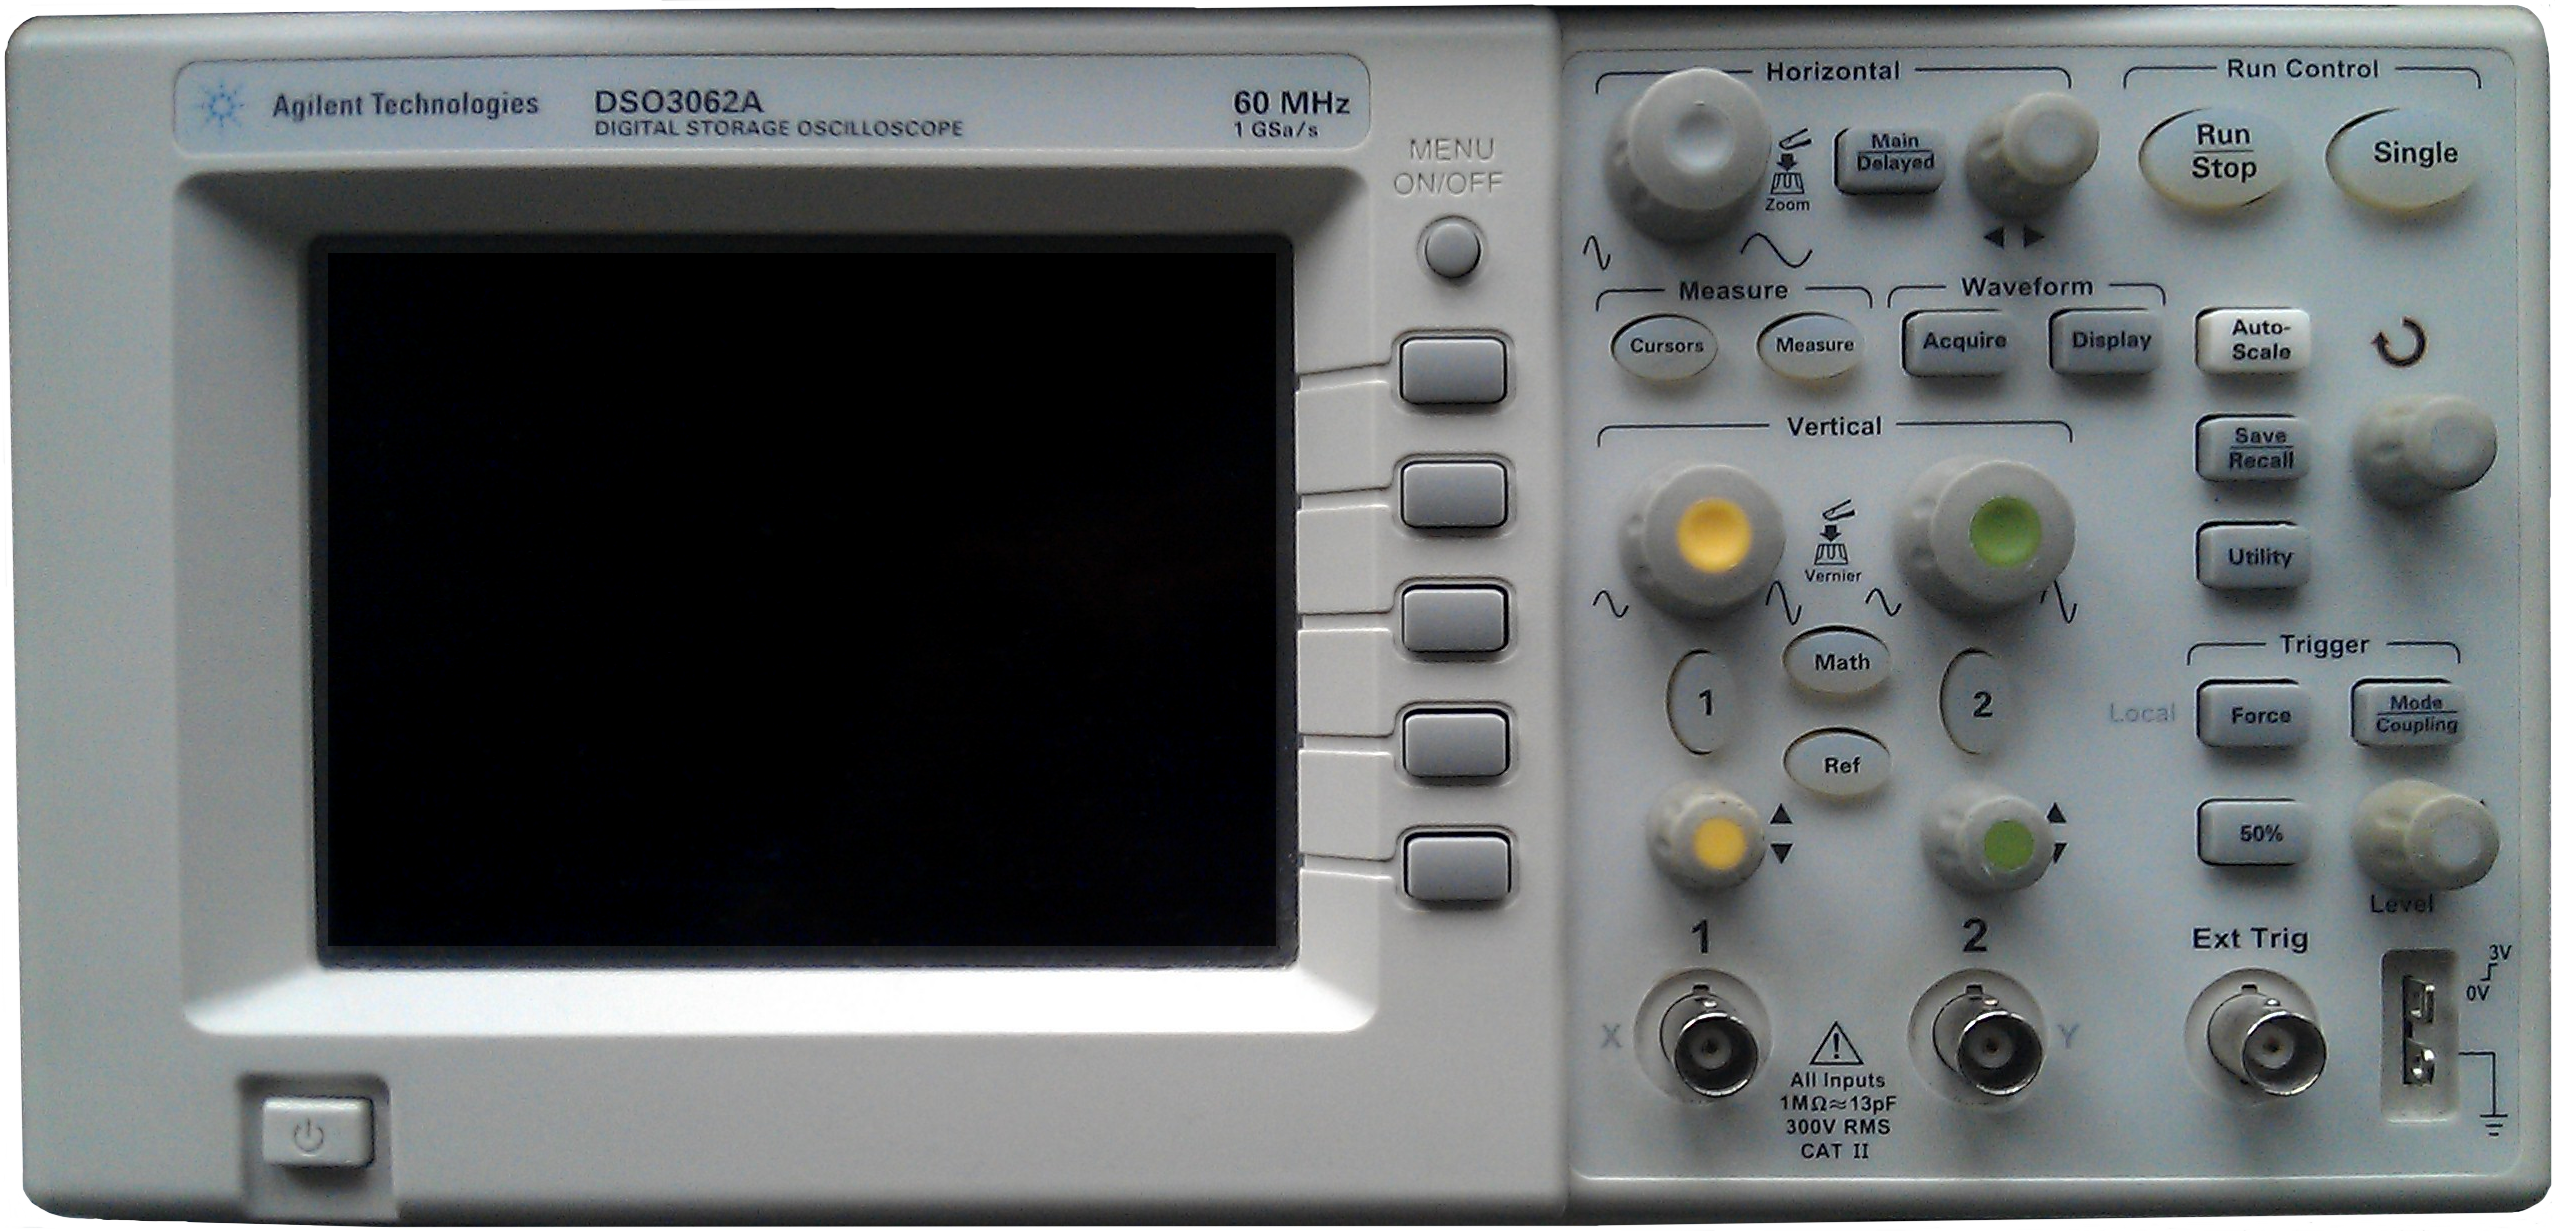
\includegraphics[scale=0.08]{Messtechnik/Bilder/oszi_foto.png}
 \vspace{-6cm}
\end{wrapfigure}

\section*{Theorie- und Prüfungsfragen} 

\mucho{1}{TJ101}
{Das Prinzip des Drespulmessgerätes berut auf}%Frage
{der Wechselwirkung der Kräfte zwischen zwei permanent magnetischen Feldern.}%A
{der Wechselwirkung der Kräfte zwischen einem magnetischen und einem elektrischen Feld.}%B
{der Wechselwirkung der Kräfte zwischen einem permanent magnetischen und einem elektromagentischen Feld.}%C
{dem erdmagentischen Feld.}%D
{C}%Lösung

\mucho{2}{TJ111}
{Mit welchem Strom zeigt ein 20-$k\Omega/V$-Instrument Vollausschlag?}%Frage
{500$\mu A$}%A
{5$mA$}%B
{50$mA$}%C
{50$\mu A$}%D
{D}%Lösung

\mucho{3}{TJ102}
{Das Drehspulmesswerk in der folgenden Schaltung hat einen maximalen Messstrom $I_M = 100\mu A$ und einen Messwerkwiderstand $R_M = 1 k\Omega$.}%Frage
{10V}%A
{50V}%B
{500V}%C
{100V}%D
{B}%Lösung


\mucho{4}{TJ805}
{Mit einem Voltmeter der Klasse 1.5, das einen Skalenendwert von 300V hat, messen Sie an einer Spannungsquelle 230V. In welchem Bereich liegt der wahre Wert?}%Frage
{Er liegt zwischen 225,5 und 234,5V.}%A
{Er liegt zwischen 226,5 und 233,5V.}%B
{Er liegt zwischen 229,5 und 230,5V.}%C
{Er liegt zwischen 229,7 und 230,3V.}%D
{A}%Lösung


\mucho{5}{TJ115}
{Ein Drehspulmessgerät hat normalerweise eine Genauigkeit von}%Frage
{ca. 1,5 \% vom Endausschlag.}%A
{ca. 0,3 \% vom Ablesewert.}%B
{ca. 0,3 \% vom Endausschlag.}%C
{ca. 0,05 \% vom Ablesewert.}%D
{A}%Lösung

\mucho{6}{TG219}
{Die richtige Oberwellenauswahl in einer Vervielfachungsstufe lässt sich am leichtesten mit einem}%Frage
{Diodentastkopf prüfen.}%A
{Absorptionsfrequenzmesser prüfen.}%B
{Universalmessgerät prüfen.}%C
{Frequenzzähler prüfen.}%D
{B}%Lösung


\mucho{7}{TJ602}
{Ein Absorptionsfrequenzmesser hat normalerweise eine Genauigkeit von}%Frage
{1 \%.}%A
{5 \%. }%B
{0,05 \%.}%C
{0,001 \%.}%D
{B}%Lösung


\mucho{8}{TJ812}
{Wie ermittelt man die Resonanzfrequenz eines passiven Schwingkreises?}%Frage
{Durch Messung von L und C und Berechnung oder z.B. mit einem Dip-Meter.}%A
{Mit einem Frequenzmesser oder einem Oszilloskop.}%B
{Mit einem Digital-Multimeter in der Stellung Frequenzmessung.}%C
{Mit Hilfe der S-Meter Anzeige bei Anschluss des Schwingkreises an den Empfängereingang.}%D
{A}%Lösung

\mucho{9}{TJ206}
{Ein Dip-Meter hat normalerweise eine Genauigkeit von etwa}%Frage
{1 \%.}%A
{10 \%.}%B
{0,05 \%.}%C
{0,001 \%.}%D
{B}%Lösung

\mucho{9}{TJ501}
{Um die Skalenendwerte einer Sende-/Empfangsanlage mit VFO mit hinreichender Genauigkeit zu überprüfen, kann man}%Frage
{einen Frequenzzähler verwenden.}%A
{ein Dipmeter verwenden.}%B
{einen Absorptionsfrequenzmesser verwenden.}%C
{ein Oszilloskop verwenden.}%D
{A}%Lösung

\mucho{10}{TJ402}
{Für welchen Zweck wird eine Stehwellenmessbrücke verwendet?}%Frage
{Zur Überprüfung der Anpassung des Senders an die Antenne}%A
{zur Frequenzkontrolle.}%B
{zur Modulationskontrolle.}%C
{als Abschluss des Senders.}%D
{A}%Lösung

\mucho{11}{TJ305}
{Welches dieser Geräte wird für die Anzeige von NF-Verzerrungen verwendet?}%Frage
{Frequenzzähler}%A
{Transistorvoltmeter}%B
{Vielfachmessgerät}%C
{Oszilloskop}%D
{D}%Lösung

\mucho{12}{TJ303}
{Um auf dem Bildschirm eines Oszilloskops ein stehendes Bild statt durchlaufender Wellenzüge zu erhalten muss, das Oszilloskop}%Frage
{eine Triggereinrichtung haben.}%A
{einen X-Vorteiler haben.}%B
{einen Y-Vorteiler haben. \vspace*{-0.06cm}}%C
{einen Frequenzmarken-Generator haben.}%D
{A}%Lösung


\section*{Praxisteil}

\subsection*{PCB mit 70cm-LPF: Bestücken \& Löten}

Bestückt und verlötet die Bauteile auf der 70cm-Platine! Beachtet beim Löten des SMDs:

\begin{itemize}
    \item als erstes ein Lötpad etwas verzinnen
    \item Zinn erwärmen und das Bauteil mit einer Pinzette darauf ablegen
    \item wenn das Bauteil plan aufliegt, abschließend das andere Pad verlöten
\end{itemize}

Berechnet eine einfache Groundplane-Antenne ($\lambda/4$) für das Band von $430
MHz$ bis $440 MHz$ und schneidet die entsprechende Länge aus einem starren
Draht. Dieser wird nun auf das Antennenpad aufgelötet.

\textbf{Hinweis}: Als Vorwiderstand verbauen wir im Kurs $470 \Omega$ um unsere
\emph{Raspberry Pi}s gegen versehentliches Kurzschließen zu schützen. Später kann dieser
gegen einen geringeren Widerstand oder sogar eine Drahtbrücke ausgetauscht
werden, um mehr Leistung an der Antenne zu erhalten. Erklärung: Der Stromfluss
wird durch den Widerstand begrenzt ($I = \frac{U}{R} = \frac{3,3 V}{470 \Omega}
\approx 7 mA$). Mit $220 \Omega$ auf $15 mA$ sollte man aber auch noch auf der
sicheren Seite sein -- "`das Internet"' berichtet von $30 mA$ am GPIO ohne
bleibende Schäden. ;-) Ist sichergestellt, dass der Filter und die Abstrahlung
an der Antenne funktionieren, kann der Widerstand auch wie gesagt weggelassen
werden. \textbf{Frage:} Welche Leistungen ergeben sich je nach Vorwiderstand
ungefähr?

\loesung{$P = U \cdot I$ \\
         $7 mA$: $3,3 V \cdot 0.007 A \approx 23 mW$ \\
         $15 mA$: $3,3 V \cdot 0.015 A \approx 50 mW$ \\
         $30 mA$: $3,3 V \cdot 0.030 A \approx 100 mW$}

\subsection*{Perfboard mit 30m-LPF: Bestücken \& Löten}

Baut einen weiteren Tiefpassfilter auf einer Lochrasterplatine auf. Beachtet,
dass diesmal \textbf{TX via GPIO 4 (Pin 7)} und ein beliebiger GND verdrahtet
werden muss (siehe Abbildung \ref{rpi}). Die Spule dient später zum Abstimmen
und soll von Hand auf einen $8mm$-Durchmesser auf ca. $1cm$ Länge gewickelt
werden -- wieviele Windungen müssen das sein?

\begin{figure}[H]
    \centering
    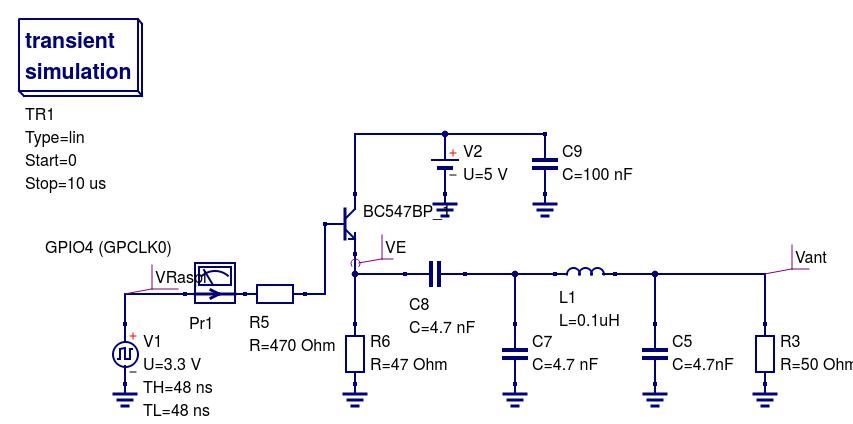
\includegraphics[width=1\textwidth]{Messtechnik/Bilder/30mRaspiAmpLP.jpg}
    \caption{Schaltung des 30m-Tiefpassfilters aus Qucs}
    \label{30mLP}
\end{figure}

\subsection*{Messprotokoll}

\begin{enumerate}
	\item Das lineare Verhalten eines Tiefpassfilters.
		\begin{itemize}
			\item Nutze die Gleichspannungsquelle und das Tischmultimeter.
			\item Lege eine Gleichspannung an den Eingang des Tiefpassfilters und messe die Ausgangsspannung.
    		\item Die Eingangspannung soll zwischen $-10~V$ und $+10~V$ liegen.
    		\item Die Eingangsspannung soll in $2~V$-Schritten geändert werden.
    		\item Um eine negative Gleichspannung mit der Gleichspannungsquelle zu realisieren, muss umgepolt werden.
    		\item Miss mit Hilfe des Tischmultimeters die Ausgangsspannung des Tiefpassfilters (Siehe Abbildung \ref{block1}).
    		\item Notiere die Messwerte direkt in Scilab, Octave oder einer Tabellekalkulation.
			\item Plotte den Verlauf der Ausgangsspannung in Abhängigkeit der Eingangsspannung.
			\item \textbf{Zusatz:} Plotten Sie den idealen Kennlinienverlauf mit in den selben Plott.
			\end{itemize}	
	\item Das Messen des Amplitudenganges eines Tiefpassfilters mit Hilfe des Oszilloskops.
		\begin{itemize}
			\item Nutze den Frequenzgenerator und das Oszilloskop.
			\item Stelle am Frequenzgenerator ein Sinus-Signal mit einer Amplitude von $10~V$ ein und lege diese an den Eingang des Tiefpassfilters.
			\item Miss mit Hilfe des Oszilloskops die Eingangs- und die Ausgangsspannung des Tiefpassfilters (Siehe Abbildung \ref{block2}).
			\item Erhöhe schrittweise die Frequenz .
			\item Nimm insgesamt 20 Messwerte auf.
			\item Verteile die Messwerte über einen Bereich von $10^1~Hz$ bis $10^4~Hz$.
			\item Verwende \texttt{$V_{RMS}$} der \texttt{Measure}-Funktion zur Messung der Amplitude
			\item Notiere die Messwerte direkt in Scilab, Octave oder einer Tabellekalkulation.
			\item Plotte den Verlauf der Amplitude (Ausgangsspannung) in Abhängigkeit der Frequenz.
			\item \textbf{Zusatz:} Stelle die Amplitude in dB dar und stelle die X-Achse auf logarthmische Darstellung um.
			\end{itemize}
	\item Das Messen der Sprungantwort eines Tiefpassfilters.
		\begin{itemize}
			\item Nutze den Frequenzgenerator und das Oszilloskop.
			\item Erzeuge mit dem Funktionsgenerator eine Rechteckfunktion mit einer Amplitude von $2,5~V$, mit einem Offset von $2,5 V$ und einer Frequenz von $5~Hz$ und lege diese an den Eingang des Tiefpassfilters.
			\item Miss mit Hilfe des Oszilloskops die Eingangs- und die Ausgangsspannung des Tiefpassfilters (Siehe Abbildung \ref{block2}).
			\item Übertrage die Sprungantwort ins Protokoll (Foto, Skizze).
			\item Hinweise zum Umgang mit dem Oszilloskop:
				\begin{itemize}
					\item Achte darauf, dass bei den einzelnen Kanälen (\textbf{CH1}, \textbf{CH2}) bei \textbf{Kopplung}: \textbf{DC} eingestellt ist.
					\item Um einwandfrei messen zu können, verwenden Sie die Trigger-Funktion des Oszilloskops. Drücken Sie die Taste \textbf{Mode/Coupling} in der Trigger-Sektion. Wählen Sie beim oberen \textbf{Modus}: \textbf{Flanke}, bei \textbf{Quelle}: \textbf{CH2}, beim unteren \textbf{Modus}: \textbf{Normal} und bei der \textbf{Kopplung}: \textbf{AC} aus.
					\end{itemize}
			\end{itemize}
 	\end{enumerate} 

\begin{figure}[H]
	\centering
	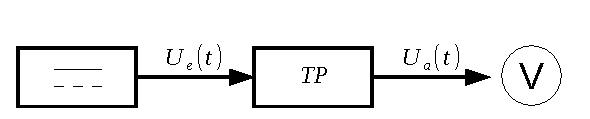
\includegraphics[scale=1]{Messtechnik/Bilder/Block_Messung_Kennlinie.pdf}
	\caption{Blcokschaltbild für die Messungen mit dem Tischmultimeter.}
	\label{block1}
	\end{figure}

\begin{figure}[H]
	\centering
	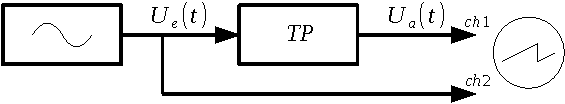
\includegraphics[scale=1]{Messtechnik/Bilder/Block_Messung_oszi.pdf}
	\caption{Blcokschaltbild für die Messungen mit dem Oszilloskop.}
	\label{block2}
	\end{figure}
